%versi 2 (8-10-2016)
\lstset{
	language=php,
	columns=fullflexible,
	showspaces=false,	
	showstringspaces=false,		
	breaklines=true,
	showlines=true, frame=single,
	tabsize=4,  
	basicstyle=\fontfamily{fvm}\selectfont, 
	commentstyle=\itshape\color{gray}, keywordstyle=\bfseries\color{blue}, 
	identifierstyle=\color{black}, stringstyle=\color{orange}	
}
\chapter{Landasan Teori}
\label{chap:teori}


Pada bab ini akan berisi landasan-landasan teori yang dipakai pada penelitian ini.

\section{Code Igniter}
\label{sec:codeigniter}


\textit{CodeIgniter}\cite{codeigniter3} adalah \textit{framework} untuk pembuatan \textit{website} yang menggunakan \textit{PHP}. \textit{CodeIgniter} mempermudah \textit{developer} untuk meminimalisir penggunaan kode untuk mengakses suatu fungsi. Seperti untuk mengambil data pada \textit{database}, mengakses file \textit{php} lainnya. Penggunaan \textit{framework CodeIgniter} juga mudah.\textit{ Developer} tidak perlu melakukan banyak konfigurasi--konfigurasi saat melakukan \textit{setup}. \textit{CodeIgniter} juga memberikan dokumentasi yang lengkap. Permasalahan \textit{routing}  sudah diselesaikan oleh \textit{framework} ini, \textit{framework} ini secara otomatis akan mengarah ke file dalam direktori \textit{controllers} sesuai dengan \textit{path-abempty} pada \textit{URI}  dan menjalankan \textit{method} \texttt{index()}.


\begin{figure}[H]
	\centering
	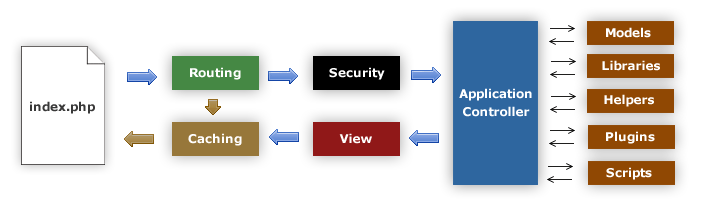
\includegraphics[scale=0.8]{mvc} 
	\caption{Flowchart MVC}
	\label{fig:appflowchart} 
\end{figure}


\textit{CodeIgniter} menerapkan arsitektur \textit{MVC} yang dapat dilihat pada gambar \ref{fig:appflowchart}, file \texttt{index.php} berfungsi mengatur routing dan mengarahkan ke \textit{application controller} yang berada di direktori \textit{controller} dan melalui \textit{controller} akan dipanggil \textit{models, libraries, helpers, etc} yang dibutuhkan dengan perintah \texttt{\$this->load}. \textit{MVC} secara umum akan mengolah data pada \textit{models} dan hasil yang sudah siap akan dikirim ke \textit{view} melalui \textit{controller}. Fitur tambahan dari arsitektur \textit{CodeIgniter} adalah saat \textit{router} memeriksa \textit{HTTP request}, jika \textit{cache} tersedia maka akan dikirimkan \textit{cache} tersebut dan jika tidak ada \textit{cache} maka \textit{security} akan memeriksa dan melakukan filter terhadap \textit{HTTP request} seperti pada gambar \ref{fig:appflowchart}. 

\subsection{Controller}

\textit{Controller} adalah pusat dari aplikasi, \textit{controller} menangani apa yang harus dilakukan dari \textit{HTTP request}. Dalam \textit{CodeIgniter} untuk menginisiasi \textit{controller} cukup menulis nama kelas diikuti dengan \texttt{extends CI\_Controller}.

\textit{CodeIgniter} secara otomatis akan menjalankan \textit{method} \texttt{index()} jika tidak diperintahkan untuk menjalankan \textit{method} tertentu. Untuk menjalankan \textit{method} lain hanya perlu ditambahkan \textit{path-abempty} seperti  \texttt{example.com/index.php/Welcome/<<nama\_method>>}.

\begin{lstlisting}
<?php
defined(`BASEPATH') OR exit(`No direct script access allowed');
	
class Welcome extends CI_Controller {
	
	public function __construct(){
		parent::_construct();
		$this->load->database();
		$this->load->model(contoh_model);
	}
	
	public function index()
	{
		$t = "hello";
		$this->load->view(`welcome_message',array(
		`t' => $t));
	}
}
\end{lstlisting}


Dalam contoh diatas dilakukan \textit{load model} dan \textit{database}. File \textit{model} akan berada di direktori \textit{model} sedangkan untuk \texttt{\$this->load->database()} akan melakukan \textit{load} pada \textit{database} menggunakan parameter yang ada pada direktori \texttt{/config/database.php}. 


\subsection{Model}

\textit{Model} berfungsi sebagai \textit{logic} dari aplikasi. \textit{ Model} pada \textit{CodeIgniter} bersifat opsional, tetapi disediakan untuk \textit{developer} yang ingin menggunakan MVC\cite{codeigniter3}. 


\begin{lstlisting}
class Blog_model extends CI_Model {
	
	public function get_last_ten_entries()
	{
		$query = $this->db->get(`entries', 10);
		return $query->result();
	}
}
\end{lstlisting}

\textit{Model} pada \textit{CodeIgniter} harus diikuti dengan \texttt{extends CI\_Model}. Hal yang berurusan terhadap \textit{database} dapat dilakukan dengan perintah \texttt{\$this->db->query(\lq<<isi query>>\rq)} atau untuk mempermudah, beberapa fungsi \textit{MYSQL} dasar disediakan oleh \textit{CodeIgniter}.\textit{ Method} bisa langsung digunakan seperti \texttt{\$this->db->get(\lq<<nama tabel>>\rq)}
untuk mengambil semua nilai dari tabel tersebut. Untuk dapat mengakses \textit{database} maka harus dipasang \textit{database} yang akan digunakan pada \texttt{config/database.php}.

\begin{lstlisting}
		
$config[`hostname'] = `localhost';
$config[`username'] = `myusername';
$config[`password'] = `mypassword';
$config[`database'] = `mydatabase';
$config[`dbdriver'] = `mysqli';
$config[`dbprefix'] = `';
$config[`pconnect'] = FALSE;
$config[`db_debug'] = TRUE;

$this->load->model(`model_name', `', $config);
\end{lstlisting}

File \texttt{database.php} diatas menyimpan kredensial dari \textit{database} yang digunakan. Mulai dari \textit{hostname, username, password dll}.

\subsection{View}


\textit{View} tidak pernah dipanggil secara langsung, \textit{view} harus dipanggil melalui \textit{controller}\cite{codeigniter3}.
\textit{View} pada \textit{CodeIgniter} ditaruh pada direktori \textit{view}. Pemanggilan \textit{view} menggunakan \textit{method} \texttt{\$this->load->view(`nama\_view')}. Jika \textit{controller} ingin mengirimkan data kepada \textit{view} maka perlu dilakukan: 

\begin{lstlisting}
$t = "hello";
$this->load->view(`welcome_message',array(`t' => $t));
\end{lstlisting}

Selanjutnya untuk menampilkan data tersebut ke halaman \textit{view}, dapat memanggil variabel \texttt{\$t}.


\subsection{Kelas pada Code Igniter}
\subsubsection{CI\_Loader}
\textit{CI\_Loader} adalah kelas yang berfungsi untuk \textit{load elements}. \textit{Elements} dapat berupa \textit{libraries, view files, drivers, helpers, models}. Kelas ini sudah diinisialisasi secara otomatis oleh \textit{code igniter}. \textit{Method} yang digunakan pada \textit{CI\_Loader}:

\begin{itemize}
	\item \texttt{library(\$library [, \$params = NULL [, \$object\_name=NULL]])} \\
	\textit{Method} ini berfungsi untuk \textit{load} kelas yang disediakan oleh \textit{codeigniter}. \\
	\textit{Parameter}: 
	\begin{itemize}
		\item \texttt{\$library}(\textit{mixed}): Nama \textit{library} dalam bentuk \textit{string}.
		\item \texttt{\$params}(\textit{array}): Parameter tambahan dalam bentuk \textit{array}.
		\item \texttt{\$object\_name}(\textit{string}): Parameter tambahan untuk mengubah nama objek.
	\end{itemize}
	\textit{Return}: \texttt{CI\_Loader}.
	\item \texttt{view(\$view [, \$vars = array() [, return=FALSE]])} \\
	\textit{Method} ini berfungsi untuk \textit{load} file \textit{view}. \\
	\textit{Parameter}:
	\begin{itemize}
		\item \texttt{\$view}(\textit{string}): Nama \textit{view}.
		\item \texttt{\$vars}(\textit{array}): Parameter tambahan berupa variabel \textit{associative array}.
		\item \texttt{\$return}(\textit{bool}): Apakah data dari tampilan dikembalikan.
	\end{itemize}
	\textit{Return}: \textit{mixed}.
	
	\item \texttt{model(\$model [, \$name ="[, \$db\_conn=FALSE]])} \\
	\textit{Method} ini berfungsi untuk \textit{load} file \textit{model}. \\
	\textit{Parameter}:
	\begin{itemize}
		\item \texttt{\$model}(\textit{mixed}): Nama \textit{model}.
		\item \texttt{\$name}(\textit{string}): Parameter tambahan untuk menamai objek\textit{model}.
		\item \texttt{\$db\_conn}(\textit{string}): Parameter tambahan untuk konfigurasi database.
	\end{itemize}
	\textit{Return}: \texttt{CI\_Loader}.
	
	\item \texttt{database([\$params="[, \$return=FALSE[,\$query\_builder=NULL]]])} \\
	\textit{Method} ini berfungsi untuk melakukan \textit{load} kelas \textit{database}. \\
	\textit{Parameter}:
	\begin{itemize}
		\item \texttt{\$params}(\textit{mixed}): Parameter tambah untuk konfigurasi dari \textit{database}. 
		\item \texttt{\$return}(\textit{bool}): Apakah mengembalikan objek \textit{database}.
		\item \texttt{\$query\_builder}(\textit{bool}): Apakah akan \textit{load} \textit{query builder}.		
	\end{itemize}
	\textit{Return}: \texttt{CI\_Loader} jika \texttt{\$return=FALSE}, \texttt{CI\_DB} jika \texttt{\$return=TRUE}.
	
	\item \texttt{config(\$file[, \$use\_sections=FALSE[, \$fail\_gracefully=FALSE]])} \\
	\textit{Method} ini akan meneruskan ke \textit{method} \texttt{\$this->config->load()}. \\ 
	\textit{Parameter}: 
	\begin{itemize} 
		\item \texttt{\$file}(\textit{string}): Nama file dari konfigurasi.
		\item \texttt{\$use\_sections}(\textit{bool}): Apakah nilai dari konfigurasi akan \textit{load} di \textit{section} sendiri.
		\item \texttt{\$fail\_gracefully}(\textit{bool}) Apakah akan mengembalikan \textit{False} jika gagal.
	\end{itemize}
	\textit{Return}: \texttt{bool}.
		
\end{itemize}

\subsubsection{CI\_Config}
\textit{CI\_Config} adalah kelas yang digunakan untuk mengambil konfigurasi yang dibuat. Kelas ini dapat digunakan dengan awalan \texttt{\$this->config}. \textit{Method} yang digunakan pada \textit{CI\_Config}: \\
\texttt{item(\$item[, \$index=''])} \\
\textit{Parameter}: 
\begin{itemize} 
	\item \texttt{\$item}(\textit{string}): Nama konfigurasi.
	\item \texttt{\$index}(\textit{string}): Nama indeks.
\end{itemize}

 
\subsubsection{CI\_Email}
\textit{CI\_Email} adalah kelas yang berfungsi untuk mempermudah pengiriman \textit{email} yang disediakan oleh \textit{codeigniter}. \textit{Load} kelas \textit{CI\_Email} dapat dilakukan dengan:
\begin{lstlisting}
$this->load->library(`email');
\end{lstlisting}
Setelah \textit{load email library} , untuk menggunakan kelas \texttt{CI\_Email} diawali dengan \texttt{\$this->email}. \textit{Method} yang digunakan pada \textit{CI\_Email}:

\begin{itemize}
	\item \texttt{from(\$from[, \$name="[, \$return\_path=NULL]])} \\
	\textit{Method} ini digunakan untuk memasang \textit{email address} dan nama dari pengirim. \\ 
	\textit{Parameter}:
	\begin{itemize}
		\item \texttt{\$from}(\textit{string}): Memasang alamat pengirim \textit{email}.
		\item \texttt{\$name}(\textit{string}): Memasang nama pengirim \textit{email}.
		\item \texttt{\$return\_path}(\textit{string}): Alamat \textit{email} tambahan jika \textit{email} gagal dikirim.
	\end{itemize}
	\textit{Return}: \texttt{CI\_Email}.
	
	\item \texttt{to(\$to)} \\
	\textit{Method} ini digunakan untuk menentukan alamat \textit{email} tujuan. \\
	\textit{Parameter}: \texttt{\$to}(\textit{mixed}), string yang dipisahkan oleh koma untuk setiap penerima atau \textit{array} dari alamat email. \\
	\textit{Return}: \texttt{CI\_Email}.
	
	\item \texttt{subject(\$subject)} \\ 
	\textit{Method} ini menulis \textit{subject} dari \textit{email}. \\
	\textit{Parameter}: \texttt{\$subject}(\textit{string}), subjek \textit{email}. \\
	\textit{Return}: \texttt{CI\_Email}.
	
	\item \texttt{message(\$body)} \\
	\textit{Method} ini digunakan menulis isi pesan. \\
	\textit{Parameter}: \texttt{\$body}(\textit{string}), \textit{email message body}. \\
	\textit{Return}: \texttt{CI\_Email}.
	
	\item \texttt{send([\$auto\_clear=TRUE])} \\
	\textit{Method} ini digunakan untuk mengirim \textit{email}. \\
	\textit{Parameter}: \texttt{\$auto\_clear}(\textit{bool}), apakah pesan akan dibuang setelah pengiriman. \\
	\textit{Return}: \textit{TRUE} jika sukses, \textit{FALSE} jika gagal.
	
	
\end{itemize}

\subsubsection{CI\_Input}
\textit{CI\_Input} adalah kelas yang digunakan untuk menyaring dan membersihkan data masukan untuk meningkatkan keamanan. Kelas ini juga menyediakan \textit{method} bantuan untuk mengambil data masukan. Kelas ini sudah diinisialisasi secara otomatis. \textit{Method} yang digunakan dari kelas \textit{CI\_Input}:
\begin{itemize}
	\item \texttt{post([\$index=NULL[, \$xss\_clean=NULL]])} \\
	Membaca masukan dengan tipe \textit{post}. \\
	\textit{Parameter}:
	\begin{itemize}
		\item \texttt{\$index}(\textit{mixed}): Parameter \textit{name}.
		\item \texttt{\$xss\_clean}(\textit{bool}): Apakah akan menggunakan \textit{XSS filtering}.
	\end{itemize}
	\textit{Return}: \texttt{\$\_POST} jika tidak ada parameter masukan, nilai dari masukan jika ditemukan, atau \textit{NULL} jika tidak ditemukan.
	
	\item \texttt{server(\$index[, \$xss\_clean=NULL ])} \\ 
	\textit{Method} ini berguna untuk mengambil \textit{server data} seperti \texttt{\$\_SERVER}. \\
	\textit{Parameter}:
	\begin{itemize}
		\item \texttt{\$index}(\textit{mixed}): \textit{Value name}. 
		\item \texttt{\$xss\_clean}(\textit{bool}): Apakah akan menggunakan \textit{XSS filtering}.
	\end{itemize}
	\textit{Return}: \texttt{\$\_SERVER} \textit{item value} jika ditemukan, \textit{NULL} jika tidak.
	
\end{itemize}

\subsubsection{CI\_Session}
\textit{Session} digunakan untuk mengurus  \textit{user's state} dan melihat aktivitas \textit{user} saat menelusuri situs. \textit{Session} sebaiknya diinisialisasi pada konstruktor di \textit{controller}. Menginisiasi \textit{session} dengan cara \texttt{\$this->load->library(\textquotesingle session\textquotesingle)}. Sedangkan penggunaannya dapat menggunakan perintah \texttt{\$this->session}. \textit{Method} yang digunakan pada kelas \texttt{CI\_Session}:

\begin{itemize}
	\item \texttt{set\_flashdata(\$data[, \$value=NULL])}	\\
	\textit{Method} ini berguna untuk menyimpan data ke \texttt{\$\_SESSION} \textit{superglobal} dan menandai sebagai \textit{flashdata}. \textit{Flashdata} adalah \textit{session data} yang hanya tersedia untuk permintaan berikutnya dan setelah itu akan dibuang.\\
	 \textit{Parameter}: 
	 \begin{itemize}
	 	\item \texttt{\$data}(\textit{mixed}): \textit{Array} dengan pasangan \textit{key/value} untuk menyimpan ke \textit{session data} atau \textit{key} jika jumlah data hanya satu. 
	 	\item \texttt{\$value}(\textit{mixed}): Nilai yang ingin disimpan jika \texttt{\$data} adalah \textit{key}.
	 \end{itemize}
	 \textit{Return}: \textit{void}.
	 
	 \item \texttt{flashdata([\$key=NULL])} \\
	 \textit{Method} ini mengambil nilai dari spesifik \texttt{\$\_SESSION} yang telah ditandai sebagai \textit{flashdata}. \\
	 \textit{Parameter}: \texttt{\$key}(\textit{mixed}), \textit{key} dari \textit{flashdata}. \\
	 \textit{Return}: Nilai dari \textit{item key} tertentu, atau \textit{array} semua \textit{flashdata}.
	
	\item \texttt{set\_userdata(\$data[, \$value=NULL])} \\
	\textit{Method} ini berguna untuk menyimpan data ke \texttt{\$\_SESSION} \textit{superglobal}. \\
	\textit{Parameter}: 
	\begin{itemize}
		\item \texttt{\$data}(\textit{mixed}): \textit{Array} dengan pasangan \textit{key/value} untuk menyimpan ke \textit{session data} atau \textit{key} jika jumlah data hanya satu.
		\item \texttt{\$value}(\textit{mixed}): Nilai yang ingin disimpan jika \texttt{\$data} adalah \textit{key}.
	\end{itemize}
	\textit{Return}: \textit{void}.
	
	\item \texttt{userdata([\$key=NULL])} \\
	\textit{Method} ini berguna untuk mengambil \textit{value} untuk \texttt{\$\_SESSION} \textit{item} atau \textit{array} semua data user jika parameter dikosongkan. \\
	\textit{Parameter}: \texttt{\$key}(\textit{mixed}), \textit{session item key} atau \textit{null}. \\
	\textit{Return}: Nilai dari \textit{item key} tertentu, atau \textit{array} semua data pengguna.
	
	\item \texttt{unset\_userdata(\$key)} \\
	\textit{Method} ini berfungsi untuk membuang data dari \texttt{\$\_SESSION} \textit{superglobal} dengan \textit{key} masukan. \\ 
	\textit{Parameter}: \$key(\textit{mixed}) \textit{key} dari \textit{session data} yang ingin dibuang. \\
	\textit{Return}:void 
	
\end{itemize}

\section{Phpspreadsheet}
\label{section:phpspreadsheet}

PhpSpreadsheet adalah \textit{library} yang ditulis dengan bahasa PHP berguna untuk membaca dan menulis file dengan jenis spreadsheet seperti Excel dan LibreOffice Calc\cite{phpspreadsheet}. Format--format yang didukung oleh phpspreadsheet dapat dilihat pada tabel \ref{tab:phpspreadsheet supported}. Pada penelitian kali ini phpspreadsheet hanya digunakan untuk menulis ke dokumen dengan \textit{extension} \texttt{.xls}

\begin{table}[H]
	\centering
	\begin{tabular}{|p{0.5\textwidth}|c|c|}
		\hline
		\textbf{Format} & \textbf{Reading} & \textbf{Writing} \\ \hline
		Open Document Format/OASIS (.ods) & \checkmark & \checkmark \\ \hline
		Office Open XML (.xlsx) Excel 2007 and above & \checkmark & \checkmark \\ \hline
		BIFF 8 (.xls) Excel 97 and above & \checkmark & \checkmark \\ \hline
		BIFF 5 (.xls) Excel 95 & \checkmark  & \\ \hline
		SpreadsheetML (.xml) Excel 2003 & \checkmark & \\ \hline
		Gnumeric & \checkmark & \\ \hline
		HTML & \checkmark & \checkmark \\ \hline
		SYLK & \checkmark & \\ \hline
		CSV & \checkmark & \checkmark \\ \hline
		PDF (using either the TCPDF, Dompdf or mPDF libraries, which need to be installed separately) & & \checkmark \\ 
		\hline
	\end{tabular}
\caption{Tabel format yang didukung oleh phpspreadsheet}
\label{tab:phpspreadsheet supported}
\end{table}

\subsection{Kelas pada Phpspreadsheet}
Pada penelitian kali ini kelas utama yang digunakan adalah kelas \textit{Spreadsheet}. Kelas \textit{Spreadsheet} dapat diakses menggunakan \texttt{use PhpOffice$\backslash$PhpSpreadsheet$\backslash$Spreadsheet}.
 \textit{Method} yang dimiliki oleh \textit{library} \textit{PhpSpreadsheet} yang digunakan pada penelitian kali ini:


\subsubsection{Spreadsheet}
	Kelas \textit{Spreadsheet} dapat diakses dengan menggunakan: 
	\begin{lstlisting}
use PhpOffice\PhpSpreadsheet\Spreadsheet;
$spreadsheet = new Spreadsheet();
	\end{lstlisting} 
	\textit{Constructor} kelas \textit{Spreadsheet} tidak menerima parameter apapun, dan \textit{return value} adalah \textit{mixed}. \textit{Method} yang digunakan pada kelas \texttt{Spreadsheet}:  
 \begin{itemize}
 	\item \texttt{createSheet([\$sheetIndex:null|int=null])} \\ 
 	\textit{Method} ini berfungsi untuk membuat \textit{sheet}.\\
 	\textit{Parameter}: \texttt{\$sheetIndex}, \textit{index} dari sheet dikosongkan jika menaruh sheet pada \textit{index} terakhir. \\ 
 	\textit{Return}: Kelas \texttt{Worksheet}.
 	
 	\item \texttt{setActiveSheetIndex(\$pIndex:int)}\\ Memilih \textit{sheet} yang ingin dijadikan \textit{active} berdasarkan \textit{index}. \\
 	\textit{Parameter}: \$pIndex, tipe data \textit{int}, \textit{index} dari \textit{Worksheet}. \\
 	\textit{Return}: Kelas \texttt{Worksheet}.
 	
 	\item \texttt{getActiveSheet()}\\
 	Mengembalikan kelas \textit{Worksheet} yang telah dibuat menjadi \textit{sheet} aktif pada \texttt{setActiveSheetIndex}.\\
 	\textit{Parameter}: Tidak ada. \\ 
 	\textit{Return}: Kelas \texttt{Worksheet}.
 \end{itemize}

\subsubsection{Worksheet}
Kelas \textit{Worksheet} adalah kelas yang mengatur nilai dari \textit{cell}, \textit{cell style}, judul \textit{sheet} dll. Pembuatan kelas ini dapat dilakukan dengan:
\begin{lstlisting}
$spreadsheet->createSheet();
\end{lstlisting}
Variabel \textit{\$spreadsheet} adalah kelas \texttt{Spreadsheet}, \textit{method} yang digunakan pada kelas \texttt{Worksheet}:

\begin{itemize}
	\item \texttt{getStyle(\$pCellCoordinate:string)} \\ 
	Mengembalikan kelas \texttt{Style}.\\
	\textit{Parameter}: \texttt{\$pCellCoordinate} koordinat dari \textit{cell} atau \textit{range}, contoh : `A1',`A1:E1'.\\
	\textit{Return}: Kelas \texttt{Style}.
	
	\item \texttt{setCellValue(\$pCoordinate : string , \$pValue : mixed )}\\ 
	mengubah suatu nilai pada \textit{cell} tertentu. \\ 
	\textit{Parameter}:
	\begin{itemize}
		\item \texttt{\$pCoordinate}: Koordinat dari \textit{cell} contoh: `A1'.
		\item \texttt{\$pValue}: Nilai baru dari \textit{cell} tersebut.
	\end{itemize}
	\textit{Return}: \texttt{\$this}.
	
	\item \texttt{mergeCells(\$pRange:string)} \\ 
	Melakukan \textit{merge} pada \textit{cell}. \\ 
	\textit{Parameter}: \texttt{\$pRange} \textit{cell range} yang ingin dilakukan \textit{merge}, contoh: `A1:E1'. \\
	\textit{Return}: \texttt{\$this}.
	\item \texttt{setTitle(\$pValue:string [, \$updateFormulaCellReferences:bool = true ] [, \\ \$validate:bool:true ] )}\\
	 Berfungsi untuk memberi judul pada \textit{sheet}. \\
	 \textit{Parameter}:
	 \begin{itemize}
	 	\item \texttt{\$pValue}: \textit{String} yang akan dijadikan nama judul.
	 	\item \texttt{\$updateFormulaCellReferences}: \textit{Flag} untuk menentukan \textit{cell reference} pada \textit{formula} akan dirubah mengikuti judul baru. Direkomendasikan untuk tidak mengubah nilai variabel ini.
	 	\item \texttt{\$validate}: Nilai asal adalah \textit{true}, pasang nilai \textit{false} untuk melewati validasi dari judul baru.
	 \end{itemize}
 	\textit{Return}: \texttt{\$this}.
	\item \texttt{getRowDimension(\$pRow:int [,\$create:bool = true ])} \\ 
	Mengambil dimensi baris pada baris tertentu. \\
	\textit{Parameter}: 
	\begin{itemize}
		\item \texttt{\$pRow}: \textit{Index} dari baris.
		\item \texttt{\$create}: Nilai \textit{default} adalah \textit{true}.
	\end{itemize}
	\textit{Return}: Kelas \texttt{RowDimension}.
	\item \texttt{getColumnDimension(\$pColumn:string [, \$create : bool = true ])} \\
	Mengambil dimensi kolom pada kolom tertentu. \\
	\textit{Parameter}:
	\begin{itemize}
		\item \texttt{\$pColumn}: String dari kolom, contoh: `A'.
		\item \texttt{\$create}: Nilai \textit{default} adalah \textit{true}.
	\end{itemize}
	\textit{Return}: Kelas \texttt{ColumnDimension}.
\end{itemize}

\subsubsection{Style}
Kelas \textit{Style} adalah kelas yang mengatur \textit{style} dari suatu \textit{cell} seperti \textit{alignment}, \textit{fill},\textit{font} dll. Kelas \textit{Style} dapat diakses menggunakan:
\begin{lstlisting}
$worksheet->getStyle(`A1');
\end{lstlisting}
Variabel \textit{\$worksheet} adalah kelas \textit{Worksheet}, \textit{method} yang tersedia pada kelas \texttt{Style}:
	\begin{itemize}
		\item \texttt{getFill()} \\
		 Mengembalikan kelas \textit{Fill}. untuk mengubah \textit{fill} pada suatu \textit{cell} dapat memanggil \texttt{set\-Fill\-Type()} pada kelas \textit{Fill}.	\\
		 \textit{Parameter}: Tidak ada.
		 \textit{Return}: Kelas \texttt{Fill}.
		\item \texttt{getAlignment()} \\
		 Mengembalikan kelas \textit{Alignment}, untuk mengubah \textit{alignment} pada suatu \textit{cell} dapat memanggil \texttt{setHorizontal()} atau \texttt{setVertical()} pada kelas \textit{Alignment}. \\
		\textit{Parameter}: Tidak ada. \\
		\textit{Return}: Kelas \texttt{Alignment}.
		\item \texttt{getFont} \\
		 Mengembalikan kelas \textit{Font}, untuk mengubah penebalan kata dapat menggunakan \texttt{setBold()} dengan masukan \textit{boolean}. \\
		\textit{Parameter}: Tidak ada. \\
		\textit{Return}: Kelas \texttt{Font}.
		
	\end{itemize}

\subsubsection{Xls} 
Kelas \texttt{Xls} memiliki 2 tipe yaitu \textit{writer} dan \textit{reader}. Pada penelitian kali ini tipe \textit{Xls} yang digunakan hanya tipe \textit{writer}. Kelas \textit{Xls} dapat diinisiasi dengan:
\begin{lstlisting}
$writer = new \PhpOffice\PhpSpreadsheet\Writer\Xls($spreadsheet);
\end{lstlisting}
\textit{Constructor} dari kelas \textit{Xls} menerima masukan berupa kelas \textit{Spreadsheet}, \textit{method} yang digunakan dari kelas \texttt{Xls}: \\
\texttt{save(\$pFilename:resource|string)}, berfungsi untuk menyimpan \textit{Spreadsheet} menjadi \textit{file}. \\
\textit{Parameter}: \texttt{\$pFilename}, menerima masukan \textit{resource} atau string. \\
\textit{Return}: \texttt{void}. 





\subsection{Instalasi Phpspreadsheet}
Sebelum dapat menginstalasi phpspreadsheet dibutuhkan composer. Composer dapat diunduh pada \url{getcomposer.org}. 


\begin{lstlisting}
composer require phpoffice/phpspreadsheet
\end{lstlisting}

perintah tersebut digunakan untuk membuat file \texttt{composer.json} dan menginstalasi \textit{dependencies} tersebut. 


\begin{lstlisting}
<?php
require `vendor/autoload.php';
use PhpOffice\PhpSpreadsheet\Spreadsheet;
$spreadsheet = new Spreadsheet();
\end{lstlisting}


Penggunaan phpspreadsheet secara dasar membutuhkan perintah \texttt{use PhpOffice$\backslash$Phpspread-\\sheet$\backslash$Spreadsheet} dan \texttt{new Spreadsheet()}.

\subsection{Contoh Penulisan Nilai pada \textit{cell}}

\textit{Phpspreadsheet} menyediakan suatu \textit{method} untuk dapat menaruh atau mengubah \textit{value} pada cell tertentu

\begin{lstlisting}
$sheet = $spreadsheet->getActiveSheet();
$sheet->setCellValue('A1', 'PhpSpreadsheet');
\end{lstlisting}

 Fungsi diatas akan menulis \lq PhpSpreadsheet \rq pada kolom \lq A1 \rq . \textit{PhpSpreadsheet} memiliki \textit{method} untuk mengubah nilai dari \textit{cell} tertentu dengan menggunakan \texttt{setCellValue('kolom','nilai')}.


\subsection{Contoh Penulisan Spreadsheet ke Xls }

\textit{Phpspreadsheet} dapat melakukan \textit{read and write} ke banyak format. Mulai dari \textit{xls,xlsx,csv} dll. Pada kali ini format yang akan digunakan adalah format  \textit{xls}.

\begin{lstlisting}
$writer = new \PhpOffice\PhpSpreadsheet\Writer\Xls($spreadsheet);
$writer->save("05featuredemo.xls");
\end{lstlisting}

Penggunaan fungsi \textit{write} dari \textit{phpspreadsheet} membutuhkan kelas \texttt{\textbackslash PhpOffice\textbackslash PhpSpread-\newline sheet\textbackslash Writer\textbackslash Xls()}. Kelas lain yang dapat digunakan untuk \textit{read}\&\textit{write} adalah \texttt{\textbackslash PhpOffice\textbackslash\\ PhpSpreadsheet\textbackslash IOFactory::createWriter(\$ spreadsheet, "Xls")}

\section{Bootstrap}
\textit{Bootstrap} adalah \textit{framework} paling terkenal untuk membuat \textit{site} yang \textit{mobile-first} dan \textit{res\-pon\-sive}\cite{bootstrap}. Dapat dilihat pada tabel \ref{tab:bootstrap mobile supported} dan tabel \ref{tab:bootstrap desktop supported}.  Hampir semua \textit{browser} pada \textit{desktop} dan \textit{mobile} dapat menjalankan \textit{bootstrap}.

\begin{table}[H]
	\centering
	\resizebox{\textwidth}{!}{
	\begin{tabular}{|l|l|l|l|l|l|}	
		\hline	
		 & \textbf{Chrome} & \textbf{Firefox} & \textbf{Safari} & \makecell[l]{\textbf{Android} \& \\ \textbf{WebView}} & \makecell[l]{\textbf{Microsoft} \\ \textbf{Edge}} \\ \hline
		\textbf{Android} & Supported & Supported & - & \makecell[l]{Android v5.0+ \\ Supported} & Supported \\ \hline
		\textbf{IOS} & Supported & Supported & Supported & - & Supported \\ \hline
		\textbf{Windows 10 Mobile} & - & - & - & - & Supported \\ \hline				
	\end{tabular}}
	\caption{\textit{Browser Mobile} yang mendukung \textit{bootstrap}}
	\label{tab:bootstrap mobile supported}
\end{table}

\begin{table}[H]
	\centering
	\resizebox{\textwidth}{!}{
		\begin{tabular}{|l|l|l|l|l|l|l|}	
			\hline	
			& \textbf{Chrome} & \textbf{Firefox}  &\makecell[l]{\textbf{Internet}\\\textbf{Explorer}} & \makecell[l]{\textbf{Microsoft}\\\textbf{Edge}} & \textbf{Opera} & \textbf{Safari} \\ 
			\hline
			\textbf{Mac} & Supported & Supported & - & Supported & Supported & Supported  \\ \hline
			\textbf{Windows} & Supported & Supported & \makecell[l]{Supported \\ IE10+} & Supported & Supported & Not supported\\ \hline		
	\end{tabular}}
	\caption{\textit{Browser Desktop} yang mendukung \textit{bootstrap}}
\label{tab:bootstrap desktop supported}
\end{table}






\subsection{Pemasangan Bootstrap}
Pemasangan dilakukan dengan cara mengunduh \textit{compiled css and jss} yang disediakan oleh \textit{bootstrap}.

\begin{lstlisting}
<head>
	<link rel = "stylesheet" href = "css/bootstrap.css">
	<script src = js/bootstrap.js></script>
</head>
\end{lstlisting}

Pemasangan \textit{bootstrap} memerlukan \textit{import} file \textit{css dan js} dari \textit{compiled bootstrap} yang telah diunduh.

\subsection{Container}
Kelas \texttt{container} adalah kelas yang dibutuhkan jika ingin menggunakan \textit{bootstrap} grid. Kelas \texttt{container} adalah kelas \textit{responsive} dan \textit{fixed-width}.
\begin{lstlisting}
<div class="container"></div>
\end{lstlisting}

\subsection{Grid} 
\textit{Grid} pada \textit{bootstrap} digunakan untuk mengatur \textit{layout} dan \textit{alignment}. \textit{Row} adalah kelas \textit{wrapper} untuk kolom. Kelas \textit{col} akan secara otomatis membagi lebar horizontal dari layout menjadi sama dapat dilihat pada gambar \ref{fig:bootstrap-grid}. Sebagai contoh 4 \texttt{col} dalam satu \textit{wrapper} akan membagi lebar masing masing menjadi 25\%. Kelas \texttt{row} mempunyai jumlah maksimum sebanyak 12. Sehingga jika ingin membagi tiga kolom dengan lebar sama dapat menggunakan \texttt{col-4}.
\begin{lstlisting}
<div class="container">
	<div class="row">
		<div class="col">
			1 of 2
		</div>
		<div class="col">
			2 of 2
		</div>
	</div>
</div>
\end{lstlisting}
Contoh gambar yang penggunaan kode diatas dapat dilihat pada gambar \ref{fig:bootstrap-grid}. Dapat dilihat bahwa kelas \texttt{col} membagi lebar horizontal menjadi sama rata. Penggunaan kelas \textit{col-6} pada dua kolom juga akan menghasilkan gambar \ref{fig:bootstrap-grid}.
\begin{figure}[H]
	\centering
	\includegraphics[scale=0.7]{bootstrap-grid}  	
	\caption[Gambar bootstrap-grid]{Gambar \textit{bootstrap-grid}}
	\label{fig:bootstrap-grid}  
\end{figure}


\subsection{Table}
Kelas \texttt{table} adalah kelas yang membantu pembuatan \textit{table}. Tambahkan \texttt{.table} pada \texttt{<table>}. Komponen--komponen yang ada pada kelas \texttt{table}:

\begin{itemize}
	\item \texttt{table-bordered} \\
	Tambahkan kelas ini jika agar semua sisi dari \textit{cell} dan \textit{table} memiliki \textit{border}.
	
	\item \texttt{table-striped} \\ 
	Tambahkan kelas ini untuk tampilan \textit{zebra-striping} di dalam \texttt{<tbody>}. Contoh penggunaan:
	\begin{lstlisting}
<table class= "table table-bordered table-striped"></table>
	\end{lstlisting}
	
	\item \texttt{table-responsive} \\ 
	Gunakan kelas ini agar tampilan horizontal tabel menjadi \textit{responsive} dan tidak \textit{overflow}. Penggunaan \texttt{table-responsive} ditaruh pada \textit{parent} dari \textit{table}. Contoh penggunaan:
	\begin{lstlisting}
<div class="table-responsive">
	<table class="table">
	...
	</table>
</div>	
	\end{lstlisting} 
\end{itemize}
\subsection{Pagination}
\textit{Pagination} dibuat menggunakan \texttt{HTML list} yang berada didalam \texttt{<nav>} untuk mengidentifikasikan \textit{pagination} sebagai bagian navigasi kepada pengguna. Bantuan pendukung yang disediakan oleh \textit{bootstrap}:

\begin{itemize}
	\item \texttt{aria-label} \\
	\texttt{aria-label} adalah suatu elemen tambahan yang berguna untuk deskripsi dari navigasi tersebut.
	\item \texttt{active} \\
	Kelas \texttt{active} digunakan untuk menandakan posisi halaman saat ini.
	\item \texttt{disabled} \\
	Kelas \texttt{disabled} digunakan untuk menonaktifkan suatu \textit{link}.
	\item \texttt{page-item} \\
	Kelas yang menandakan sebuah \textit{page item} dan ditaruh pada \textit{tag} \texttt{<li>}.
	\item \texttt{page-link} \\	
	Kelas yang menandakan sebuah \textit{item link} dan ditaruh pada \textit{tag} \texttt{<a>}.
	
\end{itemize}
Contoh penggunaan dari \textit{pagination}:
	\begin{lstlisting}
<nav aria-label="example">
	<ul class="pagination">
		<li class="page-item disabled">
			<a class="page-link" href="#" tabindex="-1">1</a>
		</li>
		<li class="page-item">
			<a class="page-link" href="#">2</a>
		</li>
		<li class="page-item">
			<a class="page-link" href="#">3</a>
		</li>
	</ul>
</nav>	
\end{lstlisting}




\subsection{Modal}
\textit{Modal} dibuat dengan \textit{html, css, javascript}. \textit{Modal} akan mengubah \textit{scroll} pada \texttt{<body>} sehingga sasaran \textit{scroll} hanya pada \textit{modal}. \textit{Modal} akan tertutup jika pengguna mengklik diluar modal. \textit{Modal} pada \textit{bootstrap} memiliki struktur yang sama, struktur \textit{modal}:

\begin{lstlisting}
<div class="modal" tabindex="-1" role="dialog">
	<div class="modal-dialog" role="document">
		<div class="modal-content">
		...
		</div>
	</div>
</div>
\end{lstlisting}

Penggunaan \textit{modal} dapat dibuat menjadi lebih rapi dengan menambahkan  \texttt{modal-header}, \texttt{modal-body}, dan \texttt{modal-footer} didalam \texttt{modal-content}.


\subsection{Form}
\textit{Bootstrap} menyediakan kelas yang dapat digunakan untuk menampilkan \textit{form} yang konsisten pada \textit{browser} ataupun \textit{smartphone}. Kelas kelas yang disediakan dan digunakan pada \textit{form}:
\begin{itemize}
	\item \texttt{form-control} \\
	Kelas ini berfungsi untuk \textit{style, focus state}, dan \textit{sizing} untuk \textit{form input} yang bersifat teks. Seperti: \texttt{<input>},\texttt{<select>}, dan \texttt{textarea}.
	
	\item \texttt{readonly} \\
	Elemen ini dapat dimasukkan pada \textit{input} untuk mencegah perubahan nilai dari \textit{input}.			
	\begin{lstlisting}
<input class="form-control" type="text"  readonly>	
	\end{lstlisting}
	
	\item \texttt{form-group} \\
	\textit{Form group} adalah kelas untuk menambah struktur pada \textit{form} dengan mengelompokkan \textit{label}, \textit{controls}, dan \textit{form validation message}. 
	
	\item \textit{Form grid} \\
	Penggunaan kelas \textit{bootstrap form} juga dapat digabungkan dengan \textit{grid} pada \textit{bootstrap}, dengan menggunakan kelas \texttt{row}. seperti:
\begin{lstlisting}
<form>
	<div class="row">
		<div class="col">
			<input type="text" class="form-control">
		</div>
		<div class="col">
			<input type="text" class="form-control">
		</div>
	</div>
</form>
\end{lstlisting}
Kode diatas akan menghasilkan \textit{form} dengan model grid seperti pada gambar \ref{fig:bootstrap-grid}.

\item \texttt{col-form-label} \\ 
Kelas \texttt{col-form-label} digunakan pada \textit{tag} \texttt{<label>} jika \textit{label} dan \textit{input} berada pada satu baris, sehingga antar \textit{label} menjadi sejajar secara vertikal, seperti pada gambar \ref{fig:horizontal-form}.
\begin{figure}[H]
	\centering
	\includegraphics[scale=0.7]{horizontal-form}  	
	\caption[Gambar bootstrap-grid]{Gambar \textit{label form} yang sejajar.}
	\label{fig:horizontal-form}  
\end{figure}

\end{itemize}


\subsection{Nav}
\textit{Nav} adalah komponen yang mengatur navigasi dengan memasukkan kelas \texttt{nav}. Kelas \texttt{nav} dibuat dengan \textit{flexbox} dan menjadi dasar untuk membuat berbagai macam navigasi. Kelas \texttt{nav} dapat ditaruh pada \textit{tag} \texttt{<nav>} atau \texttt{<ul>}. Komponen-komponen yang digunakan dari fungsi \textit{nav}:
\begin{itemize}
	\item \texttt{nav-tabs} \\
	Penggunaan kelas \texttt{nav} dan ditambahkan \texttt{nav-tabs} akan menghasilkan navigasi seperti pada gambar \ref{fig:nav-tabs}
	\begin{figure}[H]
		\centering
		\includegraphics[scale=0.7]{nav-tabs} 
		\caption{Navigasi dari \texttt{nav-tabs}}
		\label{fig:nav-tabs} 
	\end{figure}

	\item \texttt{tab-content} \\
	Penggunaan kelas \texttt{tab-content} memerlukan \textit{bootstrap.js}. Kelas ini adalah kelas pembungkus dari sekumpulan konten yang dibagi berdasarkan navigasi. Dalam gambar \ref{fig:nav-tabs} adalah bagian yang berisi sekumpulan teks.
	
	\item \texttt{tab-pane} \\
	Kelas \texttt{tab-pane} berada di dalam kelas \texttt{tab-content} yang membungkus isi konten. 
	
	\item \texttt{data-toggle} \\ 
	Atribut \texttt{data-toggle} dipasang dengan nilai \texttt{data-toggle=``tab''} agar navigasi dapat diklik untuk melakukan navigasi. Atribut ini ditaruh pada \textit{tag} \texttt{<a>} seperti:
	\begin{lstlisting}
<a class="nav-link" data-toggle="tab"></a>
	\end{lstlisting}
	
	\item \texttt{nav-item} \\
	Kelas ini digunakan pada \textit{item} dari navigasi. Contoh penggunaan:
	\begin{lstlisting}
<li class="nav-item"></li>
	\end{lstlisting}
	
	\item \texttt{nav-link} \\
	Kelas ini digunakan pada \textit{link} dari navigasi. Contoh penggunaan:
	\begin{lstlisting}
<a class="nav-link">link</a>	
	\end{lstlisting}
\end{itemize}

\subsection{Collapse}
\textit{Collapse} adalah komponen yang mengatur visibilitas dari suatu elemen. Pengunaan komponen ini harus menaruh \texttt{collapse} pada \texttt{data-toggle}. Komponen ini berguna untuk menyembunyikan atau menunjukan suatu elemen ke pengguna. Komponen pendukung yang digunakan dari \textit{collapse}:
\begin{itemize}
	\item \texttt{collapse} \\
	Kelas ini digunakan untuk menyembunyikan suatu elemen. Contoh penggunaan:
	\begin{lstlisting}
<div class="collapse" id="collapseExample">

</div>
	\end{lstlisting}
	\item \texttt{shown.bs.collapse} \\
	\textit{Event} \texttt{shown.bs.collapse} digunakan untuk melakukan suatu fungsi saat elemen terlihat oleh pengguna. \textit{Event} ini akan berjalan saat transisi CSS selesai. Contoh penggunaan:
	\begin{lstlisting}
$('#myCollapsible').on('shown.bs.collapse', function () {
	
})
	\end{lstlisting}
	
	\item \texttt{hidden.bs.collapse} \\
	\textit{Event} \texttt{hidden.bs.collapse} digunakan untuk melakukan suatu fungsi saat elemen disembunyikan dari pengguna. \textit{Event} ini akan berjalan saat transisi CSS selesai. Contoh penggunaan:
	\begin{lstlisting}
$('#myCollapsible').on('hidden.bs.collapse', function () {

})
\end{lstlisting}

\end{itemize}

\section{Google OAuth 2.0}
\textit{Google API} menggunakan \textit{OAuth 2.0 protocol}\footnote{\url{https://developers.google.com/identity/protocols/oauth2}} untuk melakukan autentikasi dan otorisasi. Untuk menggunakan \textit{OAuth 2.0} dari \textit{google} diperlukan untuk mendaftar pada \textit{google api console} untuk mendapatkan \textit{client credentials} yang dapat dibuat pada \url{https://console.developers.google.com/apis}. Setelah melakukan pembuatan \textit{project} maka di menu \textit{credentials} dapat dilakukan pembuatan \textit{OAuth client ID} seperti pada gambar \ref{fig:googleapi}.

\begin{figure}[H]
	\centering
	\includegraphics[scale=0.6]{googleapi} 
	\caption{Tampilan \textit{credentials} pada \textit{google API}}
	\label{fig:googleapi} 
\end{figure}
\section{Chart.js}



 
